\documentclass[12pt]{article}
\usepackage[paper=letterpaper,margin=1.5cm]{geometry}
\usepackage{amsmath}
\usepackage{amssymb}
\usepackage{amsfonts}
\usepackage{mathtools}
%\usepackage[utf8]{inputenc}
%\usepackage{newtxtext, newtxmath}
\usepackage{lmodern}     % set math font to Latin modern math
\usepackage[T1]{fontenc}
\renewcommand\rmdefault{ptm}
%\usepackage{enumitem}
\usepackage[shortlabels]{enumitem}
\usepackage{titling}
\usepackage{graphicx}
\usepackage[colorlinks=true]{hyperref}
\usepackage{setspace}
\usepackage{subfigure} 
\usepackage{braket}
\usepackage{color}
\usepackage{tabularx}
\usepackage[table]{xcolor}
\usepackage{listings}
\usepackage{mathrsfs}
\usepackage{stackengine}
\usepackage{physics}
\usepackage{afterpage}
\usepackage{pdfpages}
\usepackage[export]{adjustbox}
\usepackage{biblatex}

\setstackEOL{\\}

\definecolor{dkgreen}{rgb}{0,0.6,0}
\definecolor{gray}{rgb}{0.5,0.5,0.5}
\definecolor{mauve}{rgb}{0.58,0,0.82}


\lstset{frame=tb,
  language=Python,
  aboveskip=3mm,
  belowskip=3mm,
  showstringspaces=false,
  columns=flexible,
  basicstyle={\small\ttfamily},
  numbers=none,
  numberstyle=\tiny\color{gray},
  keywordstyle=\color{blue},
  commentstyle=\color{dkgreen},
  stringstyle=\color{mauve},
  breaklines=true,
  breakatwhitespace=true,
  tabsize=3
}
\setlength{\droptitle}{-6em}

\makeatletter
% we use \prefix@<level> only if it is defined
\renewcommand{\@seccntformat}[1]{%
  \ifcsname prefix@#1\endcsname
    \csname prefix@#1\endcsname
  \else
    \csname the#1\endcsname\quad
  \fi}
% define \prefix@section
\newcommand\prefix@section{}
\newcommand{\prefix@subsection}{}
\newcommand{\prefix@subsubsection}{}
\renewcommand{\thesubsection}{\arabic{subsection}}
\makeatother
\DeclareMathOperator*{\argmin}{argmin}
\newcommand{\partbreak}{\begin{center}\rule{17.5cm}{2pt}\end{center}}
\newcommand{\alignbreak}{\begin{center}\rule{15cm}{1pt}\end{center}}
\newcommand{\tightalignbreak}{\vspace{-5mm}\alignbreak\vspace{-5mm}}
\newcommand{\hop}{\vspace{1mm}}
\newcommand{\jump}{\vspace{5mm}}
\newcommand{\R}{\mathbb{R}}
\newcommand{\C}{\mathbb{C}}
\newcommand{\N}{\mathbb{N}}
\newcommand{\G}{\mathbb{G}}
\renewcommand{\S}{\mathbb{S}}
\newcommand{\bt}{\textbf}
\newcommand{\xdot}{\dot{x}}
\renewcommand{\star}{^{*}}
\newcommand{\ydot}{\dot{y}}
\newcommand{\lm}{\mathrm{\lambda}}
\renewcommand{\th}{\theta}
\newcommand{\id}{\mathbb{I}}
\newcommand{\si}{\Sigma}
\newcommand{\Si}{\si}
\newcommand{\inv}{^{-1}}
\newcommand{\T}{^\intercal}
\renewcommand{\tr}{\text{tr}}
\newcommand{\ep}{\varepsilon}
\newcommand{\ph}{\varphi}
%\renewcomand{\norm}[1]{\left\lVert#1\right\rVert}
\definecolor{cit}{rgb}{0.05,0.2,0.45}
\addtolength{\jot}{1em}
\newcommand{\solution}[1]{

\noindent{\color{cit}\textbf{Solution:} #1}}

\newcounter{tmpctr}
\newcommand\fancyRoman[1]{%
  \setcounter{tmpctr}{#1}%
  \setbox0=\hbox{\kern0.3pt\textsf{\Roman{tmpctr}}}%
  \setstackgap{S}{-.9pt}%
  \Shortstack{\rule{\dimexpr\wd0+.1ex}{.9pt}\\\copy0\\
              \rule{\dimexpr\wd0+.1ex}{.9pt}}%
}

\newcommand{\Id}{\fancyRoman{2}}
\addbibresource{citations.bib}


% Enter the specific assignment number and topic of that assignment below, and replace "Your Name" with your actual name.
\title{STAT 31020: Homework 4}
\author{Caleb Derrickson}
\date{January 31, 2024}

\begin{document}
\onehalfspacing
\maketitle
\allowdisplaybreaks
\tableofcontents

\newpage
\section{Problem 1}
We aim to understand both trust-region approaches and sparsity of matrices. 
\subsection{Problem 1, part 1}
For the Rosenbrock function of order n we used in last homework,\\
$f(x) = \sum_{i = 1}^{n - 1} \left[ 100 (x_{i+1} - x_i^2)^2 + (x_i - 1)^2\right]$
implement a function to return the sparse Hessian.
\partbreak
\begin{solution}

    I have just added the condition that the returned hessian is sparse. I passed the dense matrix to the sparse() function provided by Matlab.
\end{solution}

\newpage
\subsection{Problem 1, part 2}
We will experiment with sparse and dense linear algebra. Let $b \in \R^n$ be a vector of ones of dimension n. Compute the Hessian $H$ at the point of all entries being equal to 2. Solve the equation $Hx = b$ and time it for $H$ being sparse format and denote the time by a(n) with dense format and denote the time by b(n) using the backslash operator. Plot a(n) and b(n) as functions of n. what seems to be the rough behavior of a(n) and b(n)? 
\partbreak
\begin{solution}

    The plot is given as Figure \ref{fig:MatMult}. I tried fitting polynomials to both plots and I got that the dense matrix time scales roughly by $n^2$ (the coefficient of $n^3$ is of the order $10^{-11}$; for $n^2$, $10^{-8}$), while the sparse matrix scales roughly by $n$ (the coefficient of $n^2$ is of order $10^{-10}$; for $n$, $10^{-7}$). 
\end{solution}
\vspace{4cm}
\begin{figure}[!h]
    \centering
    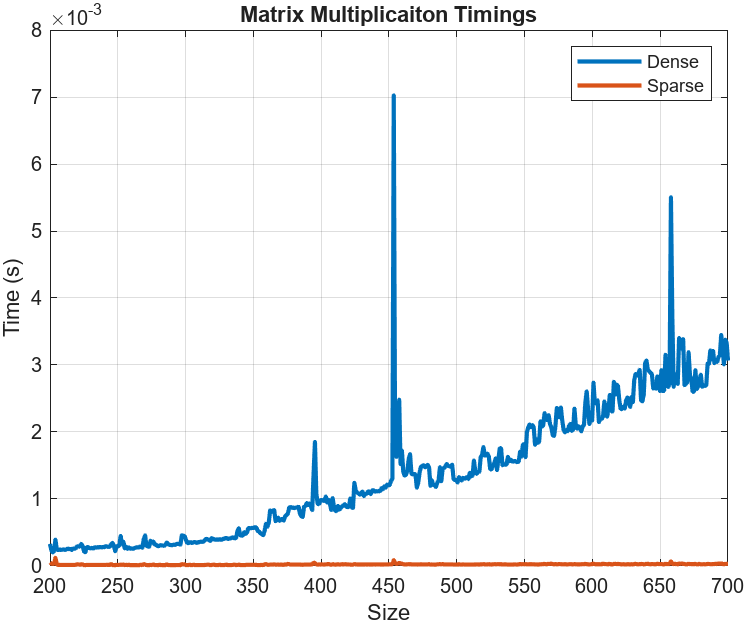
\includegraphics[width = 0.5\textwidth]{Plots/MatrixMultiplicationTimings.png}
    \caption{Solving $Ax = b$ for $A$ dense vs sparse and the given Hessian.}
    \label{fig:MatMult}
\end{figure}

\newpage
\subsection{Problem 1, part 3}
Write a program that implements the dogleg trust-region approach. Experiment with the parameters or by designing your own rules. Report the total number of linear systems solved and the total number of funciton evaluations.

\newpage
\section{Problem 2}

\newpage
\section{Problem 3}
\newcommand{\alphabar}{\overline{\alpha}}
We will show that steepest descent with backtracking has asymptotic linear convergence. Let $x_k$ be a sequence produced by steepest descent with line search and backtracking when applied to the nonlinear optimization problem $\min_{x} f(x)$, where the function $f(x)$ is three times continuously differentiable. This is the algorithm you implemented in the second homework except you will apply it to a general function. In particular, we will assume that backtracking is initialized at a fixed stepsize $\alphabar$ as we did in problem 2 in homework 2. Assume that $x_k \rightarrow x\star$ where $x\star$ satisfies the second order sufficient conditions. 

\subsection{Problem 3, part a}
Prove that there exists a neighborhood of $x\star$ and parameters $0 < c_1 < c_2$ such that $c_1 \norm{\grad f(x)}^2 \leq f(x) - f(x\star) \leq \norm{\grad f(x)}^2$ for any $x$ within the neighborhood $N(x\star)$.
\partbreak

\begin{solution}

    The first inequality can be shown as follows. We first note that the neighborhood $N(x\star)$ can be chosen around $x\star$ such that $f(x \in N(x\star))$ is convex, as well as the gradient $\grad f(x)$ is Lipshchitz. Note that \cite{zhou2018fenchel} gives\footnote{This result is [5] on page 4. I have two choices concerning this: I can either give my own, sloppier version of the proof; or I can cite the reference itself. I feel it is more transparent that I cite it.}. 
    \[f(y) \geq f(x) + \grad f(x)\T (y - x) + \frac{1}{2L}\norm{\grad f(y) - f(x)}^2, \quad \forall x, y.\]
    This result is directly applicable when we restrict $x, y \in N(x\star)$, so that we can assure convevity of $f$ and Lipschitzness of $\grad f$. Substituting $y \mapsto x$ and $x \mapsto x\star$ gives,
    \[f(x) \geq f(x\star) + \grad f(x\star)\T (x - x\star) + \frac{1}{2L}\norm{\grad f(x) - \grad f(x\star)}^2.\]
    By the second order sufficient conditions, we have that $\grad f(x\star) = 0$, so we get 
    \[\frac{1}{2L}\norm{\grad f(x)}^2 \leq f(x) - f(x\star).\]
    So we have $c_1 = \frac{1}{2L}$. To find the second inequality, we can approximate the function $f(x)$ for some $x \in N(x\star)$, 
    \[f(x) = f(x\star) + \grad f(x\star)(x - x\star) + \frac{1}{2}(x - x\star)\T \grad^2 f(x\star)(x - x\star).\]
    By the second order sufficient conditions we have $\grad f(x\star) = 0$, so with rearranging, we have
    \[f(x) - f(x\star) = \frac{1}{2}(x - x\star)\T \grad^2 f(x\star)(x - x\star)\]
    The right hand side can be bounded by Cauchy Schwartz to give
    \[f(x) - f(x\star) \leq \norm{x - x\star}^2 \norm{\grad^2f(x\star)}.\]
    By problem 3 part a of Homework 2 we found 
    \[c'\norm{x - x\star} \leq \norm{\grad f(x)},\]
    for some $c' > 0.$ We can substitute this into our inequality to get
    \[f(x) - f(x\star) \leq \frac{1}{2(c')^2} \norm{\grad^2f(x\star)}\norm{\grad f(x)}^2.\]
    Therefore, setting $c_2 = \frac{1}{2(c')^2}\norm{\grad^2 f(x\star)}$, we have found the following chain of inequalities to be found.  
\end{solution}

\newpage
\subsection{Problem 3, part b}
In the case where $f(x)$ is quadratic,
$f(x) = f + g\T x + \frac{1}{2}x\T Bx,$ $ B\succ 0$ find the sharpest values of $c_1, c_2$ as a function of the eigenvalues of $B$. Prove that they are the sharpest by finding $x \neq x\star$, where the inequalities above are, in effect, equalities.
\end{document}